\documentclass[a4paper]{article}
\usepackage{amsmath}
\usepackage{amsthm}
\usepackage[english]{babel}
\usepackage[utf8]{inputenc}
\usepackage{graphicx}
\usepackage[colorinlistoftodos]{todonotes}

\title{3D Cuboid Labeling}

\author{Leo}

\date{\today}
\begin{document}
\maketitle

%\begin{abstract}
%This paper will state and prove the quadratic formula.
%\end{abstract}

\section{Introduction}
Given an image, we want to recover the inherent 3D structure behind it.
For simplicity, we often treat the scene as a cuboid. Such approximation is quite enough for applications such as environment map generation.
To label each face of the cuboid, we should firstly set up the 3 axes, as Figure~\ref{fig1} shows.
$p_0$ is the intersection of the 3 axes and the vector $\overrightarrow{p_0p_1}$, $\overrightarrow{p_0p_2}$ and $\overrightarrow{p_0p_3}$ indicate the direction of $x$, $y$ and $z$.
So how do we get the 3D positions of these points based on those projected coordinates in 2D?
\begin{figure}[h]
\centering
%\begin{tabular}{c}
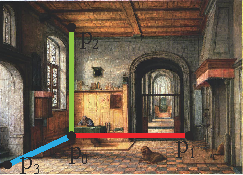
\includegraphics[width=1.0\linewidth]{images/fig.pdf}
%\end{tabular}
\caption{A image with labeled axes.}
\label{fig1}
\end{figure}


\section{Inference}
\label{sec:inference}
Assume the width and height of the image are $w$ and $h$ respectively. The focal length of the camera is $f$.
Applying the projection transformation to a 3D point $[X,Y,Z]$, we get
\begin{equation}
 \begin{bmatrix}2f/w & 0 & 0 & 0 \\0 & 2f/h & 0 & 0\\ 0 & 0 & a & b\\ 0 & 0 & -1 & 0 \end{bmatrix}  \begin{bmatrix}X\\Y\\Z\\1 \end{bmatrix} =
 \begin{bmatrix} 2fX/w\\2fY/h\\aZ+b\\-Z \end{bmatrix} \sim \begin{bmatrix} -2fX/(wZ)\\-2fY/(hZ)\\-(aZ+b)/Z\\1 \end{bmatrix},
\end{equation}
where $a = -\frac{F+N}{F-N}$, $b = -\frac{2FN}{F-N}$, $F$ and $N$ are the near and far plane.
The 2D position $[u,v]=[-2fX/(wZ), -2fY/(hZ)]$ is the projected coordinate of $[X,Y,Z]$.
The labeled 2D position $[u,v]$ is known, so we have
\begin{align}
X&=(-\frac{w}{2f})uZ \label{equ:X}\\
Y&=(-\frac{h}{2f})vZ\label{equ:Y}.
\end{align}
Back to Figure~\ref{fig1}, assume the 2D position of the labeled point is $p_k=[u_k,v_k]$ and the corresponding 3D position is $P_K=[X_k,Y_k,Z_k]$.
With $\overrightarrow{p_0p_1} \perp \overrightarrow{p_0p_2}$, we have
\begin{equation}
(X_1-X_0)(X_2-X_0)+(Y_1-Y_0)(Y_2-Y_0)+(Z_1-Z_0)(Z_2-Z_0)=0\label{equ:prep}.
\end{equation}
Substituting Equation~\ref{equ:X} and~\ref{equ:Y} into~\ref{equ:prep}:
\begin{align}
(\frac{w}{2f})^2(u_1Z_1-u_0Z_0)(u_2Z_2-u_0Z_0)+ & \nonumber\\
(\frac{h}{2f})^2(v_1Z_1-v_0Z_0)(v_2Z_2-v_0Z_0)+ & \nonumber\\
(Z_1-Z_0)(Z_2-Z_0) &=0,
\end{align}
or
\begin{align}
(\frac{w}{2f})^2(u_1u_2Z_1Z_2-u_0u_2Z_0Z_2-u_0u_1Z_0Z_1+u_0^2Z_0^2)+ & \nonumber\\
(\frac{h}{2f})^2(v_1v_2Z_1Z_2-v_0v_2Z_0Z_2-v_0v_1Z_0Z_1+v_0^2Z_0^2)+ & \nonumber\\
(Z_1Z_2-Z_0Z_2-Z_0Z_1+Z_0^2) &=0\label{equ:complex}.
\end{align}
Define $C_{mn}=(\frac{w}{2f})^2u_mu_n+(\frac{h}{2f})^2v_mv_n+1$ and substitute it to Equation~\ref{equ:complex}:
\begin{equation}
C_{12}Z_1Z_2-C_{02}Z_0Z_2-C_{01}Z_0Z_1+C_{00}Z_0^2=0,
\end{equation}
i.e.
\begin{equation}
(C_{12}Z_2-C_{01}Z_0)Z_1=(C_{02}Z_2-C_{00}Z_0)Z_0 \label{equ:sym1}.
\end{equation}
Symmetrically, we also have
\begin{align}
(C_{23}Z_3-C_{02}Z_0)Z_2&=(C_{03}Z_3-C_{00}Z_0)Z_0 \label{equ:sym2} \\
(C_{31}Z_1-C_{03}Z_0)Z_3&=(C_{01}Z_1-C_{00}Z_0)Z_0 \label{equ:sym3}.
\end{align}
According to Equation~\ref{equ:sym3}, $Z_3=\frac{(C_{01}Z_1-C_{00}Z_0)Z_0}{C_{31}Z_1-C_{03}Z_0}$.
Substituting it back to Equation~\ref{equ:sym2}, we can express $Z_2$ using $Z_0$ and $Z_1$.
Then Substituting $Z_2$ into Equation~\ref{equ:sym1} (I use Matlab for such tedious work), we get
\begin{align}
(C_{01}^2C_{23}-C_{01}C_{03}C_{12}-C_{01}C_{02}C_{31}+C_{00}C_{12}C_{31})Z_1^2 & +\nonumber\\
(C_{01}C_{02}C_{03}-C_{00}C_{01}C_{23}+C_{01}C_{02}C_{03}-C_{00}C_{01}C_{23})Z_1Z_0 & + \nonumber\\
C_{00}^2C_{23}-C_{00}C_{02}C_{03})Z_0^2&=0.
\end{align}
Solving such a quadratic equation, we get $Z_1$.
Finally there are 2 sets of solution for Equation~\ref{equ:sym1}~-~\ref{equ:sym3}.
We can choose either one.

\end{document}


